%% bare_conf.tex
%% V1.4b
%% 2015/08/26
%% by Michael Shell
%% See:
%% http://www.michaelshell.org/
%% for current contact information.
%%
%% This is a skeleton file demonstrating the use of IEEEtran.cls
%% (requires IEEEtran.cls version 1.8b or later) with an IEEE
%% conference paper.
%%
%% Support sites:
%% http://www.michaelshell.org/tex/ieeetran/
%% http://www.ctan.org/pkg/ieeetran
%% and
%% http://www.ieee.org/

\documentclass[conference]{IEEEtran}

% *** GRAPHICS RELATED PACKAGES ***
\usepackage[pdftex]{graphicx}
% declare the path(s) where your graphic files are
% \graphicspath{{../pdf/}{../jpeg/}}
% and their extensions so you won't have to specify these with
% every instance of \includegraphics
% \DeclareGraphicsExtensions{.pdf,.jpeg,.png}

% *** MATH PACKAGES ***
\usepackage{amsmath}

% *** PDF, URL AND HYPERLINK PACKAGES ***
\usepackage{url}

% Links entre imagens, citações e urls.
\usepackage{hyperref}

% A codificação deste documento está em UTF-8.
\usepackage[utf8]{inputenc}
% Hifenização do texto e tradução de palavras como Abstract, Section, etc.
\usepackage[brazil]{babel}
% Hifenização de palavras acentuadas.
\usepackage[T1]{fontenc}

% correct bad hyphenation here
\hyphenation{op-tical net-works semi-conduc-tor}


\begin{document}
\title{Utilizando Spatial Transformer Networks}


\author{\IEEEauthorblockN{Lucas Caetano Possatti}
\IEEEauthorblockA{Universidade Federal do Espírito Santo\\
Email: lucas.cpossatti@gmail.com}
\and
\IEEEauthorblockN{Rafael Horimoto de Freistas}
\IEEEauthorblockA{Universidade Federal do Espírito Santo\\
Email: rafael.hdefreitas@gmail.com}}

% make the title area
\maketitle

\begin{abstract}
Redes Neurais Convolucionais (CNNs) estão sendo muito utilizadas para alcançar resultados do estado da arte na área de Visão Computacional. Uma propriedade desejável para tais modelos, que lidam com imagens, é serem capazes de desassociar posicionamento e deformações de objetos e de características da imagem. Assim sendo, tais modelos podem se tornar invariantes espacialmente ou até mesmo usarem a informação desassociada para ajudar na tarefa de inferência.
Para alcansar tal propriedade, é explorado nesse trabalho, baseado no trabalho de Jaderberg et al \cite{jaderberg2015spatial}, o uso de \textit{Spatial Transformer Networks} (STNs). STNs são módulos que podem ser incluídos em outras redes neurais, provendo capacidades de transformação espacial, e podem ser usados juntamente com o algoritmo de backpropagation.
\end{abstract}


% For peerreview papers, this IEEEtran command inserts a page break and
% creates the second title. It will be ignored for other modes.
\IEEEpeerreviewmaketitle

\section{Introdução}

Redes Neurais Convolucionais (CNNs) estão sendo muito utilizadas para alcançar resultados do estado da arte na área de Visão Computacional. Uma propriedade desejável para tais modelos, que lidam com imagens, é serem capazes de desassociar posicionamento e deformações de objetos e de características da imagem. Assim sendo, tais modelos podem se tornar invariantes espacialmente ou até mesmo usarem a informação desassociada para ajudar na tarefa de inferência.
Certa invariância espacial pode ser obtida através de camadas de \textit{max-pooling} local. Porém, devido ao tipicamente pequeno espaço no qual o \textit{max-pooling} atua, tal invariância só é alcansada após um profunda hierarquia de convoluções e camadas de \textit{max-pooling}, de forma que as camadas intermediárias não são invariantes a largas transformações nos dados de entrada.
Para alcansar tal propriedade, é explorado nesse trabalho, baseado no trabalho de Jaderberg et al \cite{jaderberg2015spatial}, o uso de \textit{Spatial Transformer Networks} (STNs). STNs são módulos que podem ser incluídos em outras redes neurais, provendo capacidades de transformação espacial, e podem ser usados juntamente com o algoritmo de backpropagation. A STN pode ter como entrada uma imagem ou um mapa de características, inferi uma transformação condicionada a entrada e aplica a transformação na entrada para obter a saída.
A STN é dividida em três partes: rede de localização, gerador de malha e amostrador. A rede de localização aprende os parâmetros de uma transformação condicionados à entrada da STN. O gerador de malha então usa os parâmetros aprendidos pela rede de localização para transformar a malha de pixels da saída. A malha de pixels transformada defini as coordenadas correspondentes na entrada, porém tais coordenadas podem não ser inteiras, o que impossibilita definir diretamente cada pixel de saída em função de um único pixel de entrada. Para tratar tal problema, o amostrador usa as coordenadas da malha transformada juntamente com os pixels de entrada e aplica um algoritmo de mapeamento de textura para gerar os pixels de saída.

\section{Trabalhos Correlatos}

Segundo Jaderberg et al. \cite{jaderberg2015spatial}, trabalhos anteriores modelam transformações com redes neurais \cite{hinton1981parallel,hinton2011transforming,tieleman2014optimizing}, aprendem e analisam representações invariantes a transformações \cite{bruna2013invariant,cohen2014transformation,gens2014deep,kanazawa2014locally,lenc2015understanding,sohn2012learning} e usam mecanismos de atenção e detecção para seleção de características \cite{ba2014multiple,erhan2014scalable,girshick2014rich,gregor2015draw,schmidhuber1991learning,sermanet2014attention}.
Trabalho anterior por Hinton \cite{hinton1981parallel} visava atribuir frames canônicos de referência para partes de objetos, um tema que repercurtiu em \cite{hinton2011transforming} onde transformações afins 2D foram modeladas para criar um modelo generativo composto de partes transformadas. Os alvos do esquema de treino generativo são as imagens de entrada transformadas, com as transformações entre imagens de entrada e alvos dadas como entrada adicional para a rede. O resultado é um modelo generativo que consegue aprender a gerar imagens transformadas de objetos compondo partes. A noção de composição de partes transformadas é levada a frente por Tieleman \cite{tieleman2014optimizing}, onde partes aprendidas são explicitamente transformadas por transformações afins, com a transformação inferida pela rede. Tais modelos generativos são capazes de aprender características discriminativas para classificação com supervisão de transformações.
A invariância e equivariância de representações de CNNs em relação a transformações de imagens de entrada são estudadas em \cite{lenc2015understanding} estimando as relações lineares entre representações das imagens originais e transformadas. Cohen \& Welling \cite{cohen2014transformation} analizam esse comportamento em relação a grupos simétricos, que também é explorado na arquitetura proposta por Gens \& Domingos \cite{gens2014deep}, resultando em mapas de características que são mais invariantes a grupos simétricos. Outras tentativas de criar representações invariantes a transformações são \textit{scattering networks} \cite{bruna2013invariant}, e CNNs que constroem bancos de filtros com filtros transformados \cite{kanazawa2014locally,sohn2012learning}.
Stollenga et al. \cite{stollenga2014deep} usa uma política baseada em ativações de uma rede para reunir as respostas dos filtros da rede para uma subsequente passagem da mesma imagem e então permitir atenção para características específicas. Nesse trabalho, é focado alcansar representações invariantes manipulando os dados em vez dos extratores de características, algo que foi feito para agrupamento em \cite{frey2002fast}.
Redes neurais com atenção seletiva manipulam os dados fazendo recortes, e então são capazes de aprender invariância a translação. Trabalhos como \cite{ba2014multiple,sermanet2014attention} são treinados com aprendizado de reforço para evitar a necessidade de um mecanismo de atenção diferenciável, enquanto [14] usa um mecanismo de atenção diferenciável usando kernels gaussianos em um modelo generativo. O trabalho por Girshick et al. \cite{girshick2014rich} usa um algoritmo de proposição de região como uma forma de atenção, e \cite{erhan2014scalable} mostra que é possível fazer regressão de regiões salientes com uma CNN. O modelo apresentado nesse trabalho pode ser visto como uma generalização de atenção diferenciável para qualquer transformação espacial.

\section{Metodologia}

Para a realização dos experimentos utilizamos um computador com Ubuntu 14.04.4 LTS e três placas de vídeo GeForce GTX 660. O código para a realização dos experimentos pode ser encontrado no \href{https://github.com/possatti/mestrado-dl-stn}{repositório deste projeto}.

Neste trabalho nós realizamos alguns experimentos aplicando redes neurais em versões distorcidas do MNIST e do CIFAR-10. A versão distorcida do MNIST, nós chamamos de Cluttered MNIST (CM). E criamos imagens distorcidas do CIFAR-10 (C10) através de scripts próprios, e o chamamos de CIFAR-10-DISTORTED (C10D).
A seguir, explicamos mais detalhadamente esses datasets.

\subsection{Cluttered MNIST}

\begin{figure}[ht!]
  \centering
  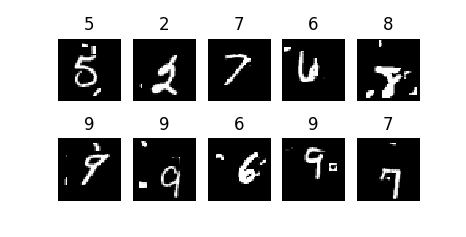
\includegraphics[width=250px]{img/CM-samples.png}
  \caption{Exemplos de imagens do  Cluttered MNIST. A classe de cada exemplo está acima do mesmo.}
  \label{fig:cm-samples}
\end{figure}

O Cluttered MNIST que usamos pode ser encontrado em \footnote{\url{https://github.com/daviddao/spatial-transformer-tensorflow/raw/master/data/mnist_sequence1_sample_5distortions5x5.npz}}. O dataset foi construído utilizando as imagens do MNIST original, porém com translações aleatórias e adição de ruído (\textit{clutter}) em cada imagem. Infelizmente não temos detalhes sobre os parâmetros usados para a criação desse dataset. Alguns exemplos de imagens do Cluttered MNIST são apresentadas na Figura~\ref{fig:cm-samples}. Neste dataset cada imagem está na resolução de $40\times40$ píxeis, com um único canal.
E o dataset é dividido em 10000 imagens para treino; 1000 para validação; e 1000 para teste.
Este é o mesmo dataset utilizado no experimento do modelo de pesquisa de STN do Tensorflow\footnote{\url{https://github.com/tensorflow/models/tree/master/research/transformer}}.



\subsection{CIFAR-10-DISTORTED}

O CIFAR-10\footnote{\url{https://www.cs.toronto.edu/~kriz/cifar.html}} é um dataset que consiste de 60000 imagens RGB de $32\times32$ píxeis. Cada imagem pertencendo a uma de dez classes possíveis, com 6000 imagens para cada classe. O dataset está divido em 50000 imagens para treino e 10000 imagens para teste.

\begin{figure}[ht!]
  \centering
  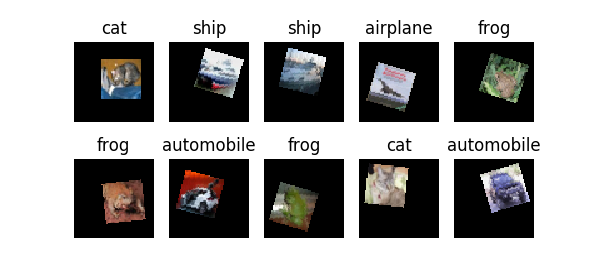
\includegraphics[width=250px]{img/C10D-samples.png}
  \caption{Exemplos de imagens do CIFAR-10-DISTORTED. A classe de cada exemplo está acima do mesmo.}
  \label{fig:c10d-samples}
\end{figure}

Utilizando as imagens do CIFAR-10 nós criamos imagens distorcidas do mesmo ao aplicar rotação, e translação às imagens, visando criar um dataset de imagens distorcidas que chamamos de CIFAR-10-DISTORTED. O processo para a criação de uma imagem distorcida pode ser compreendido pelo seguinte processo: criamos um canvas preto $64\times64$ píxeis e colamos a imagem do CIFAR-10 ($32\times32$ píxeis) no centro; aplicamos uma rotação aleatória no intervalo de $[-20, 20]$ graus; aplicamos uma translação aleatória em $X$ e outra em $Y$ no intervalo de $[-10, 10]$ píxeis. Alguns exemplos de imagens do CIFAR-10-DISTORTED são apresentados na Figura~\ref{fig:c10d-samples}

Utilizando esse método criamos um \textit{batch} de imagens de teste fixo, salvo em disco. Já para o treino, nós utilizamos o mesmo processo para gerar distorções aleatórias nas imagens de treino ``\textit{on the fly}''.

A divisão entre imagens de treino e teste foi mantida. Ou seja, 50000 imagens de treino e 10000 imagens de teste. Porém, 10\% das imagens de treino foram aleatoriamente selecionadas para compor um conjunto de validação, que não participou do treino (i.e. não foram utilizadas para atualizar os pesos da rede).

\section{Experimentos}

Nós utilizamos dois modelos de redes neurais em nossos testes: Baseline e STN. Ambas são Redes Neurais Convolucionais (CNN), a única diferença entre os dois modelos está no fato de que a STN tem uma \textit{Spatial Transformer Layer} como primeira camada da rede. Em todos os outros aspectos as redes são idênticas. A composição dessas duas redes variam para cada um dos datasets. A Tabela~\ref{tab:locnet-comp} mostra a composição da rede de localização (LocNet) utilizada no \textit{Spatial Transformer} das STNs (em ambos os datasets). A Tabela~\ref{tab:cm-comp} mostra a composição do Baseline para o Cluttered MNIST. A Tabela~\ref{tab:c10-comp} mostra a composição do Baseline para o CIFAR-10 e CIFAR-10-DISTORTED.

A notação que nós utilizamos para descrever as camadas das redes é a seguinte.
$\text{Conv2D}[K, N, A]$ é uma camada convolucional 2D onde: $K$ é o tamanho do kernel; $N$ é o número de kernels; $A$ é a função de ativação utilizada.
$\text{FC}[N, A]$ é uma camada totalmente conectada, onde: $N$ é o número de neurônios; $A$ é a função de ativação.
Em $\text{MaxPooling}[P]$, $P$ é o tamanho do \textit{cluster} do \textit{pooling}.

\begin{table}[!ht]
  \begin{center}
    \begin{tabular}{|c|}
      \hline
      \textbf{LocNet}                              \\ \hline
      $\text{MaxPooling}[2\times2]$                \\ \hline
      $\text{Conv2D}[5\times5, 20, \text{Linear}]$ \\ \hline
      $\text{MaxPooling}[2\times2]$                \\ \hline
      $\text{Conv2D}[5\times5, 20, \text{Linear}]$ \\ \hline
      $\text{FC}[50, \text{ReLU}]$                 \\ \hline
      $\text{FC}[6, \text{Linear}]$                \\ \hline
    \end{tabular}
  \end{center}
  \caption{Composição do rede de localização usada nas STNs.}
  \label{tab:locnet-comp}
\end{table}

\begin{table}[!ht]
  \begin{center}
    \begin{tabular}{|c|}
      \hline
      \textbf{CM Baseline}                       \\ \hline
      $\text{Conv2D}[3\times3, 32, \text{ReLU}]$ \\ \hline
      $\text{MaxPooling}[2\times2]$              \\ \hline
      $\text{Conv2D}[3\times3, 32, \text{ReLU}]$ \\ \hline
      $\text{MaxPooling}[2\times2]$              \\ \hline
      $\text{FC}[256, \text{ReLU}]$              \\ \hline
      $\text{FC}[10, \text{Softmax}]$            \\ \hline
    \end{tabular}
  \end{center}
  \caption{Composição do Baseline usado no Cluttered MNIST (CM).}
  \label{tab:cm-comp}
\end{table}

\begin{table}[!ht]
  \begin{center}
    \begin{tabular}{|c|}
      \hline
      \textbf{C10 Baseline}                       \\ \hline
      $\text{Conv2D}[3\times3, 48, \text{ReLU}]$  \\ \hline
      $\text{Conv2D}[3\times3, 48, \text{ReLU}]$  \\ \hline
      $\text{MaxPooling2D}[2\times2]$             \\ \hline
      $\text{Conv2D}[3\times3, 96, \text{ReLU}]$  \\ \hline
      $\text{Conv2D}[3\times3, 96, \text{ReLU}]$  \\ \hline
      $\text{MaxPooling2D}[2\times2]$             \\ \hline
      $\text{Conv2D}[3\times3, 192, \text{ReLU}]$ \\ \hline
      $\text{Conv2D}[3\times3, 192, \text{ReLU}]$ \\ \hline
      $\text{MaxPooling2D}[2\times2]$             \\ \hline
      $\text{FC}[512, \text{ReLU}]$               \\ \hline
      $\text{FC}[256, \text{ReLU}]$               \\ \hline
      $\text{FC}[10, \text{Softmax}]$             \\ \hline
    \end{tabular}
  \end{center}
  \caption{Composição do Baseline usado no CIFAR-10 (C10) e CIFAR-10-DISTORTED.}
  \label{tab:c10-comp}
\end{table}



\section{Resultados}

Nessa seção discutimos os resultados obtidos através da execução dos experimentos.

\subsection{Resultados no Cluttered MNIST}

\begin{figure}[ht!]
  \centering
  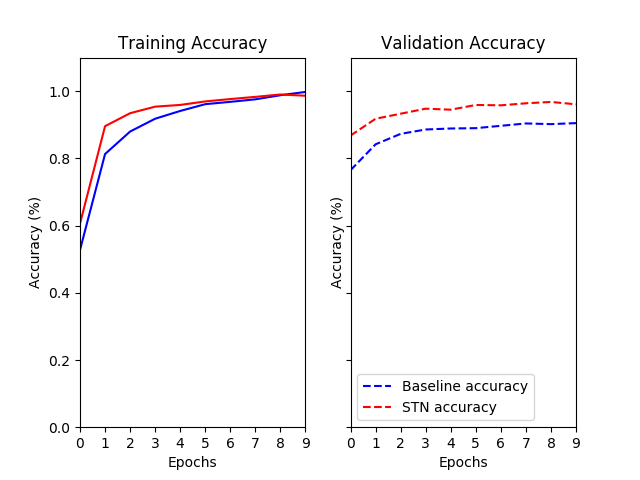
\includegraphics[width=250px]{img/CM-training-accs.png}
  \caption{Acurácias de treino (esquerda) e validação (direita) ao longo do treinamento no Cluttered MNIST.}
  \label{fig:cm-training-accs}
\end{figure}

A Figura~\ref{fig:cm-training-accs} mostra a acurácia dos modelos ao longo do treino (10 épocas). É possível notar que os dois modelos alcançam acurácias de treinamento muito próximas, porém acurácias de validação bem distintas. Com a STN obtendo um desempenho melhor que o Baseline. Isso se confirma ao executarmos os modelos no conjunto de teste, veja a Tabela~\ref{tab:cm-teste-accs}. Observamos que a STN obteve 6 pontos percentuais a mais que o Baseline quanto a acurácia no conjunto de testes.

\begin{table}[!ht]
  \begin{center}
    \begin{tabular}{|l|l|}
      \hline
      \textbf{Modelo} & \textbf{Acurácia} \\ \hline
      Baseline        & 0.90              \\ \hline
      STN             & 0.96              \\ \hline
    \end{tabular}
  \end{center}
  \caption{Acurácia dos modelos nas imagens de teste do Cluttered MNIST.}
  \label{tab:cm-teste-accs}
\end{table}

\begin{figure}[ht!]
  \centering
  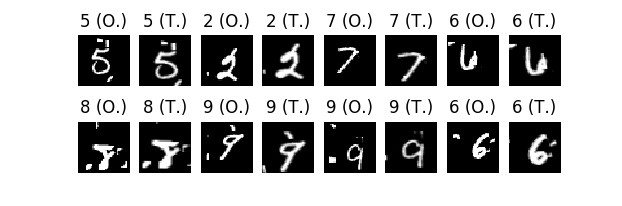
\includegraphics[width=250px]{img/CM-through-st.png}
  \caption{Exemplos de imagens transformadas pelo Spatial Transformer. Acima de cada imagem está a classificação correta, seguida de um marcador que diz se a imagem é original (O.) ou transformada (T.).}
  \label{fig:cm-through-st}
\end{figure}

Na Figura~\ref{fig:cm-through-st} podemos ver alguns exemplos de imagens transformadas pela \textit{Spatial Transformer} da STN. Na Figura, as imagens originais do dataset estão lado a lado com as suas respectivas versões transformadas. Observando as transformações, poderíamos dizer que a ST aprendeu a escalar e centralizar os dígitos de forma a apresentar o dígito de maneira mais normalizada para o restante da rede. Vemos também alguns exemplos de imagens  que provavelmente se beneficiariam de rotação. Porém não notamos qualquer sinal de que a rede tenha aprendido a rotacionar os dígitos.
% Talvez porque essa transformação, na prática, não beneficiaria a classificação.

\subsection{Resultados no CIFAR-10-DISTORTED}

Além de executar os experimentos no CIFAR-10-DISTORTED, executamos também no CIFAR-10 (usando os mesmo modelos). A Figura~\ref{fig:c10-training-accs} mostra a acurácia de treinamento e validação ao longo de 20 épocas de treino.

\begin{figure}[ht!]
  \centering
  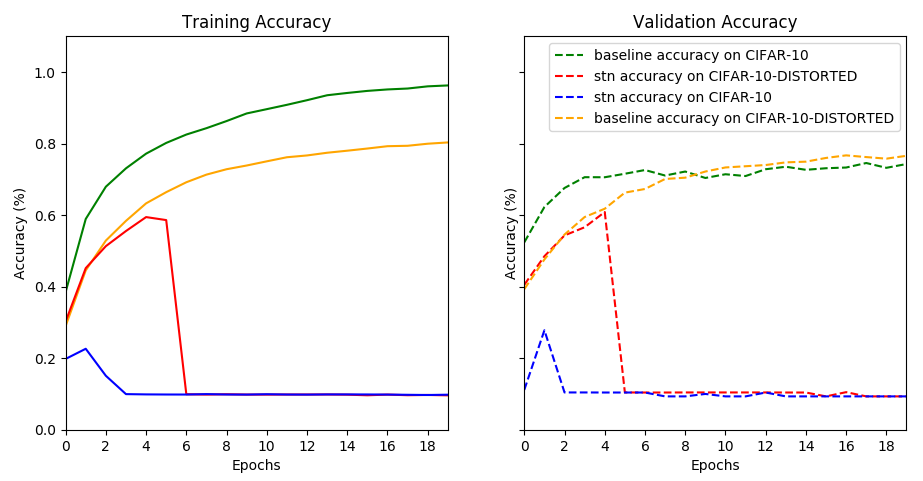
\includegraphics[width=250px]{img/C10-training-accs.png}
  \caption{Acurácias de treino (esquerda) e validação (direita) ao longo do treinamento no CIFAR-10 e CIFAR-10-DISTORTED.}
  \label{fig:c10-training-accs}
\end{figure}

Podemos notar que após algumas épocas de treinamento a qualidade da STN piorou drasticamente. Investigando o problema, passamos algumas imagens do CIFAR-10-DISTORTED através do \textit{Spatial Transformer} do modelo treinado, e obtivemos imagens completamente pretas. Isso nos leva a conjecturar que, após algum tempo de treinamento, a rede de localização se perde de forma que o foco do \textit{Spatial Transformer} fica totalmente nas regiões pretas da figura e não consegue recuperar o foco na imagem colorida de forma alguma. Não entendemos exatamente porque isso aconteceu, mas pensamos que talvez poderíamos ter amenizado ou contornado esse problema adotando uma das seguintes estratégias: diminuindo a \textit{Learning Rate}; utilizando um agendamento da \textit{Learning Rate} (como é feito no artigo da STN); ou utilizando uma rede de localização mais robusta (mais parâmetros). Infelizmente não tivemos tempo para abordar essas possibilidades e realizar mais experimentos.

A Tabela~\ref{tab:c10-teste-accs} mostra a acurácia dos modelos treinados.

\begin{table}[!ht]
  \begin{center}
    \begin{tabular}{|l|l|l|}
      \hline
      \textbf{Dataset} & \textbf{Modelo} & \textbf{Acurácia} \\ \hline
      CIFAR-10           & Baseline & 0.74 \\ \hline
      CIFAR-10           & STN      & 0.1  \\ \hline
      CIFAR-10-DISTORTED & Baseline & 0.56 \\ \hline
      CIFAR-10-DISTORTED & STN      & 0.1  \\ \hline
    \end{tabular}
  \end{center}
  \caption{Acurácia dos modelos no conjunto de testes do CIFAR-10 e CIFAR-10-DISTORTED.}
  \label{tab:c10-teste-accs}
\end{table}

\section{Conclusão}

O Spatial Transformer é um módulo construído para adicionar invariância espacial as CNNs. Ele faz isso ao aplicar uma transformação na imagem de entrada com objetivo de trazer foco ao objeto de interesse. Através dos experimentos que realizamos no \textit{Cluttered MNIST} nós pudemos observar o funcionamento do ST e os resultados que ele pode trazer para o modelo. Realizamos também um segundo experimento nos datasets CIFAR-10 e CIFAR-10-DISTORTED, mas os modelos foram gravemente prejudicados pelo uso do ST, por motivos que não pudemos identificar por completo.


% conference papers do not normally have an appendix

% trigger a \newpage just before the given reference
% number - used to balance the columns on the last page
% adjust value as needed - may need to be readjusted if
% the document is modified later
%\IEEEtriggeratref{8}
% The "triggered" command can be changed if desired:
%\IEEEtriggercmd{\enlargethispage{-5in}}

% references section

% can use a bibliography generated by BibTeX as a .bbl file
% BibTeX documentation can be easily obtained at:
% http://mirror.ctan.org/biblio/bibtex/contrib/doc/
% The IEEEtran BibTeX style support page is at:
% http://www.michaelshell.org/tex/ieeetran/bibtex/
%\bibliographystyle{IEEEtran}
% argument is your BibTeX string definitions and bibliography database(s)
%\bibliography{IEEEabrv,../bib/paper}
%
% <OR> manually copy in the resultant .bbl file
% set second argument of \begin to the number of references
% (used to reserve space for the reference number labels box)

% \begin{thebibliography}{1}

% \bibitem{IEEEhowto:kopka}
% H.~Kopka and P.~W. Daly, \emph{A Guide to \LaTeX}, 3rd~ed.\hskip 1em plus
%   0.5em minus 0.4em\relax Harlow, England: Addison-Wesley, 1999.

% \end{thebibliography}

\bibliography{bibliography}
\bibliographystyle{ieeetr}

\end{document}


